%%%%%%%%%%%%%%%%%%%%%%%%%%%%%%%%%%%%%%%%%%%%%%%%%%%%%%%%%%%%%%%%%%%%%%%%%%%%%%%%
%2345678901234567890123456789012345678901234567890123456789012345678901234567890
%        1         2         3         4         5         6         7         8

\documentclass[letterpaper, 10 pt, conference]{ieeeconf}  % Comment this line out
                                                          % if you need a4paper
%\documentclass[a4paper, 10pt, conference]{ieeeconf}      % Use this line for a4
                                                          % paper

\IEEEoverridecommandlockouts                              % This command is only
                                                          % needed if you want to
                                                          % use the \thanks command
\overrideIEEEmargins
% See the \addtolength command later in the file to balance the column lengths
% on the last page of the document

\usepackage{graphicx}
\usepackage{float}
\usepackage{graphics}
\usepackage[utf8]{inputenc}
\usepackage[spanish, activeaccute]{babel}
\usepackage{mathtools}
\usepackage{amsmath}


% Para los acentos
%\usepackage[spanish]{babel}
% The following packages can be found on http:\\www.ctan.org
%\usepackage{graphics} % for pdf, bitmapped graphics files
%\usepackage{epsfig} % for postscript graphics files
%\usepackage{mathptmx} % assumes new font selection scheme installed
%\usepackage{times} % assumes new font selection scheme installed
%\usepackage{amsmath} % assumes amsmath package installed
%\usepackage{amssymb}  % assumes amsmath package installed

\title{\LARGE \bf
Laboratorio 1 - Control Automático II - Ing. Electrónica
}

%\author{ \parbox{3 in}{\centering Huibert Kwakernaak*
%         \thanks{*Use the $\backslash$thanks command to put information here}\\
%         Faculty of Electrical Engineering, Mathematics and Computer Science\\
%         University of Twente\\
%         7500 AE Enschede, The Netherlands\\
%         {\tt\small h.kwakernaak@autsubmit.com}}
%         \hspace*{ 0.5 in}
%         \parbox{3 in}{ \centering Pradeep Misra**
%         \thanks{**The footnote marks may be inserted manually}\\
%        Department of Electrical Engineering \\
%         Wright State University\\
%         Dayton, OH 45435, USA\\
%         {\tt\small pmisra@cs.wright.edu}}
%}

\author{Ignacio Nahuel Chantiri 69869/1 \\ Thomas Jorge Sille 68373/6\\ %\vspace{1cm}
{\it Universidad Nacional De La Plata, Argentina.}}                              % <-this % stops a space

\begin{document}

\maketitle
\thispagestyle{empty}
\pagestyle{empty}


%%%%%%%%%%%%%%%%%%%%%%%%%%%%%%%%%%%%%%%%%%%%%%%%%%%%%%%%%%%%%%%%%%%%%%%%%%%%%%%%
\begin{abstract}

Estas instrucciones son una guía b\'asica para la preparaci\'on de un informe y un ejemplo de formato predefinido que puede ser usado como plantilla.

El Resumen debe enunciar concisamente qu\'e fue hecho, c\'omo fue hecho, resultados principales, y su trascendencia. No debe contener ecuaciones, figuras, tablas, o referencias. 


\end{abstract}


%%%%%%%%%%%%%%%%%%%%%%%%%%%%%%%%%%%%%%%%%%%%%%%%%%%%%%%%%%%%%%%%%%%%%%%%%%%%%%%%
\section{Introducci\'on}

El laboratorio se centra en la implementación de la técnica de control por realimentación de estados.


\section{Marco teórico}


\subsection{Identificación de Bloques y sus funciones de transferencia.}
Se presenta a continuación el circuito con los distintos bloques identificados.

\begin{figure}[H]
  \centering
  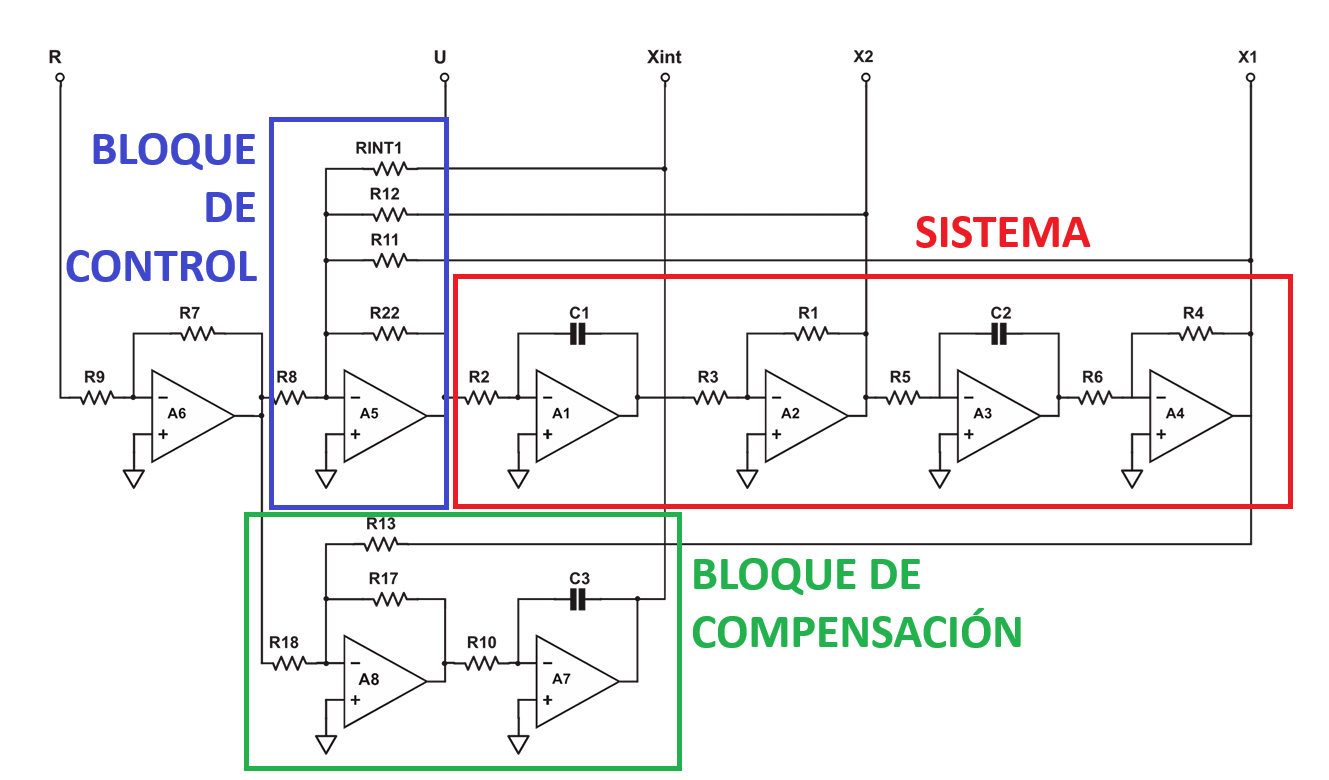
\includegraphics[width=0.43\textwidth]{IDENTIFICACION DE VLOQUES.png}
  \caption{Diagrama del circuito con los distintos bloques identificados}
  \label{fig:diag_elect_esq}
\end{figure}

\begin{itemize}
     \item \textbf{Sistema:} Compuesto por dos integradores. Para compensar la inversión asociada a la etapa de integración, se utilizan también dos inversores, uno a la salida de cada integrador. Tiene como entrada $U$, y $X1$ como salida.\\

     
    
          $\begin{cases}
            X_2 = \frac{U}{C_1R_2s}             \\
            X_1 = \frac{U}{(C_1R_2s)(C_2R_5s)}  \\
            \end{cases}$ \\ \\
        
        
     Se obtiene:
     
     \begin{equation}
        \frac{X_1}{U} = \frac{1}{(C_1R_2)(C_2R_5)s^2}  \\
        \end{equation}

    Reemplazando por los valores reales, y teniendo en cuenta que $R_{2}C_{1} = R_{5}C_{2}$:
    
    \begin{equation}
        \frac{X_1}{U} = \frac{10.000}{s^2}  \  \  [seg^2] \\
        \end{equation}
    
     \item \textbf{Bloque de control:} Lo compone un sumador con una ganancia distinta para cada valor de entrada. Su salida es $U$, y sus entradas, $X_1$, $X_2$ y $X_{int}$

     \begin{equation}
        U = R - \frac{R_{22}}{R_{int}}X_{int} - \frac{R_{22}}{R_{12}}X_{2} - \frac{R_{22}}{R_{11}}X_{1}   \  \  [] \\
        \end{equation}
    Expresado de este modo, quedan en evidencia las 3 distintas transferencias del bloque, dependiendo de cada entrada. \\
    
     \item \textbf{Bloque de compensación:} El bloque resta el valor de referencia $-R$ con la salida $X1$, y luego integra esta diferencia o error. Su salida es $X_{int}$.
     
     \begin{equation}
        X_{int} = \frac{-(R-X_{1})}{{sR_{10}}C_{3}}    \  \  [] \\
        \end{equation}

\end{itemize}




\subsection{Bloques y sus sistemas de variables de estado}
El sistema representado por sus variables de estado $x$ = ($x_1$ ,$x_2$), se halla expresado en la forma:
\[
\begin{aligned}
\dot{x} &= Ax + BU \\
 y &= Cx + DU
\end{aligned}
\]
Para el bloque \textit{Sistema}, las matrices correspondientes son:
\\
\[ 
A = \begin{bmatrix}
0 & \frac{1}{R_5C_2} \\
0 & 0
\end{bmatrix}, \quad
B = \begin{bmatrix}
0 \\
\frac{1}{R_2C_1}
\end{bmatrix}, \quad 
C = \begin{bmatrix}
0 & 1
\end{bmatrix}, \quad
D = 0
\] 

\begin{figure}[H]
  \centering
  \includegraphics[width=0.43\textwidth]{bloque sistema.png}
  \caption{Diagrama del bloque Sistema}
  \label{fig:diag_elect_esq}
\end{figure}

Para el bloque de \textit{Compensación}, teniendo en cuenta que el bloque inversor tiene ganancia 1, obtenemos un sistema de una sola variable de estado, $X_{int}$. Para un entendimiento más claro, se decidió representar el sistema no en forma matricial, sino como ecuacion diferencial:

 \begin{equation}
        \frac{dX_{\text{int}}}{dt} = \frac{R}{R_{10}C_3} - \frac{Y}{R_{10}C_3}  \\
        \end{equation}

\begin{figure}[H]
  \centering
  \includegraphics[width=0.43\textwidth]{Bloque errores.png}
  \caption{Diagrama del bloque de compensación de error}
  \label{fig:diag_elect_esq}
\end{figure}


\subsection{Análisis de Controlabilidad} 
Previamente obtuvimos las matrices A y B:

\[ 
A = \begin{bmatrix}
0 & \frac{1}{R_5C_2} \\
0 & 0
\end{bmatrix}, \quad
B = \begin{bmatrix}
0 \\
\frac{1}{R_2C_1}
\end{bmatrix}, \quad 
\] 

Llevándolas a la Forma Canónica Controlable mediante el cambio de variables $x_1 = x_1R_5C_2$, $x_2 =x_2R_5C_5$, resulta:

\[ 
A = \begin{bmatrix}
0 & 1\\
0 & 0
\end{bmatrix}, \quad
B = \begin{bmatrix}
0 \\
1
\end{bmatrix}, \quad 
C = \begin{bmatrix}
0 & A
\end{bmatrix}, \quad
D = 0
\] 

Se evidencia ahora la controlabilidad del sistema, pues las ecuaciones de estado son:

\[
\begin{aligned}
\dot{x_1} &=  x_2 \\
\dot{x_2}&= U \\
\end{aligned}
\]
Donde la entrada $U$ controla $\dot{x_2}$, por lo que controla $x_2$. \\
A su vez, $x_2$ controla $\dot{x_1}$, por lo que también controla $x_1$
De esta manera, se accede a todas las variables de estado mediante la entrada $U$, lo que demuestra la controlabilidad del sistema.

\subsection{Análisis de Observabilidad}

Podemos obtener la Forma Canónica Observable partiendo de la forma Canónica Controlable, sabiendo que

\[
\begin{aligned}
A_{c}^{T} &=  A_{o} \\
B_{c}^{T} &=  C_{o} \\
\end{aligned}
\]

Donde el subíndice $c$ indica forma controlable y $o$ forma observable.
De esta forma obtenemos $A_{o}$ y $C_{o}$, presentados a continuación:

\[ 
A = \begin{bmatrix}
0 & 0\\
1 & 0
\end{bmatrix}, \quad
C = \begin{bmatrix}
0 & 1
\end{bmatrix} \quad 
\] 

Y las ecuaciones de estado son:

\[
\begin{aligned}
\dot{x_2} &=  x_1 \\
y&= x_2 \\
\end{aligned}
\]

El análisis de observabilidad es análogo, mediante Y. \\
La salida Y es observable, por lo que $x_2$ es observable. \\
Al ser $x_2$ conocida, también lo es $\dot{x_2}$. \\
Finalmente, a través de $\dot{x_2}$  observamos $x_1$ \\
\subsection{Ejemplo del uso de Referencias}

El principio de superposici\'on es v\'alido para cualquier red resistiva lineal ~\cite{c7}. Si hay $N$ fuentes independientes debemos efectuar $N$ experimentos, cada uno con s\'olo una de las fuentes independientes activas y las otras inactivas.

\section{Desarrollo experimental}



\section{Resultados y discusi\'on}

Presentar y describir aqu\'i los resultados obtenidos a partir del experimento. Analizarlos y contrastar a partir del marco te\'oírico. Comparar resultados y determinar la magnitud de los errores y sus posibles causas, sacar conclusiones al respecto, etc. Usar gráficos y/o tablas dependiendo del tipo de resultado que se quiere mostrar y referenciarlas.

%%%%%%%%%%%%%%%%Tabla simple
\begin{table}[h]
\begin{center}
\begin{tabular}{|c||c|}
\hline
Propiedad & Valor\\
\hline
Corriente [A]& 4.9\\
\hline
Tensi\'on [V]& 218\\
\hline
\end{tabular}
\end{center}
\caption{Descripci\'on de la Tabla}
\label{tab:simple}
\end{table}

En el texto principal se har\'a referencia a cada una de las tablas explicando su contenido. La Tabla \ref{tab:simple} muestra un ejemplo de tabla simple generada en LaTeX, en tanto la Tabla \ref{tab:compleja} es un ejemplo m\'as complejo que une celdas de varias filas y columnas. 

%%%%%%%%%%%%%%%%Tabla compleja
\begin{table}[!h]
\begin{center}
\begin{tabular}{|l|c|c|}
\cline{2-3}
\multicolumn{1}{c}{}& \multicolumn{2}{|c|}{Datos} \\
\cline{2-3}
\multicolumn{1}{c|}{}& Propiedad & Valor \\
\hline \cline{2-3} {$t_1$} & Corriente  & 5.3 A \\
\cline{2-3}
                      & Tensi\'on    & 220 V\\
\hline \cline{2-3} {$t_2$} & Corriente  & 4.9 A \\ \cline{2-3}
                     & Tensi\'on    & 218 V\\
\hline
 \end{tabular}
 \end{center}
 \caption{Valores observados de corriente y voltaje en distintos instantes de tiempo $t_i$.}
 \label{tab:compleja}
\end{table}


%%%%% Figure
\begin{figure}[htp]
\centering
\includegraphics[width=0.43\textwidth]{Fig.jpg}
\caption{Magnetizaci\'on como funci\'on del campo aplicado.
Note que la leyenda de la figura est\'a centrada en la columna. } 
\label{fig:fig}
\end{figure}

Como ejemplo de formato para las figuras podemos ver la Fig.\ref{fig:fig} en donde se obserba el valor de magnetizaci\'on en funci\'on del campo magn\'etico aplicado. Los puntos representan los valores obtenidos experimentalmente en tanto que la l\'inea continua se corresponde con el ajuste realizado para tal conjunto de puntos.  

\section{Conclusiones}

Dependiendo de las caracter\'isticas del trabajo, de los datos analizados o del sistema estudiado las discusiones pueden presentarse en una secci\'on final o incluirse en la presentaci\'on de los resultados. No es una secci\'on estrictamente requerida. Aunque puede ser \'util como un repaso de los puntos m\'as importantes del trabajo, no debe ser una replica del Resumen. Debe elaborarse para destacar la importancia del trabajo realizado presentado, para sugerir cambios, mejoras, aplicaciones o extensiones futuras.
 

\addtolength{\textheight}{-12cm}   % This command serves to balance the column lengths
                                  % on the last page of the document manually. It shortens
                                  % the textheight of the last page by a suitable amount.
                                  % This command does not take effect until the next page
                                  % so it should come on the page before the last. Make
                                  % sure that you do not shorten the textheight too much.

%%%%%%%%%%%%%%%%%%%%%%%%%%%%%%%%%%%%%%%%%%%%%%%%%%%%%%%%%%%%%%%%%%%%%%%%%%%%%%%%



%%%%%%%%%%%%%%%%%%%%%%%%%%%%%%%%%%%%%%%%%%%%%%%%%%%%%%%%%%%%%%%%%%%%%%%%%%%%%%%%



%%%%%%%%%%%%%%%%%%%%%%%%%%%%%%%%%%%%%%%%%%%%%%%%%%%%%%%%%%%%%%%%%%%%%%%%%%%%%%%%
\section*{Ap\'endice}


\section*{A.  Algunas convenciones sobre formato}

En esta secci\'on se describen en m\'as detalle algunas convenciones sobre el formato del informe en general.

\subsection*{A.1     Lenguaje}

Es sumamente importante entender que un trabajo cient\'ifico o un informe t\'ecnico debe tener un tenor objetivo y formal, por lo tanto se recomienda evitar apreciaciones subjetivas y expresiones coloquiales en el mismo. Tenga en cuenta que el sentido de ciertas palabras o expresiones en el lenguaje coloquial puede ser completamente distinto al que tiene tienen t\'ecnicamente. 

Preste atenci\'on a la redacci\'on del texto; no es s\'olo una cuesti\'on de formalidad del lenguaje, sino fundamentalmente de presentar un trabajo que sea claro y entendible, sin renunciar a la rigurosidad de lo que se expone. En este sentido, es fundamental una gram\'atica correcta. As\'i mismo, los errores ortogr\'aficos restan claridad y seriedad a cualquier trabajo. La omisi\'on del acento escrito o la mala utilizaci\'on de los mismos es un error ortogr\'afico grave. Revise y corrija su trabajo antes de presentarlo.

\subsection*{A.2		Ecuaciones}

Las ecuaciones deben ser tratadas como parte de una oraci\'on (estando o no en l\'inea), es decir, deben est\'a seguidas de punto, coma, etc, como en
\begin{equation}
     a + b = c.
\end{equation}\label{ec:ejemplo}

Para los s\'imbolos, utilice It\'alicas. Todas las variables y par\'ametros involucrados en la ecuaci\'on deben estar definidos en el texto antes de que la misma sea presentada o inmediatamente despu\'es. Enumere las ecuaciones consecutivamente con el n\'umero de ecuaci\'on entre par\'entesis al mismo nivel en el margen derecho, como en la Ec.~(1). La ecuaci\'on se referencia en el texto como Ec.~(1), Ecs.~(1) y (2), etc., excepto en el comienzo de una oraci\'on: ``La ecuaci\'on (1) es...", ``...como se desprende de la Ec.~(1)."


 \subsection*{A.3		Figuras y Tablas}

A diferencia de las ecuaciones, las figuras y tablas no se consideran parte del texto. Pueden flotar sobre el texto y ser acomodadas donde mejor queden despu\'es de que son referenciadas en el texto. La forma de referenciarlas es escribiendo Fig. 1, Figs. 1, Fig. 1 (a) o Tabla I, seg\'un sea el caso. Todas las figuras y tablas deben estar referenciadas en el texto en donde se har\'a una discusi\'on de lo que se esquematiza en las mismas o los resultados que se presentan. 

Deben tener una resoluci\'on 'aceptable' como para poder apreciarse lo que se quiere mostrar. En el caso de gr\'aficos, los ejes deben est\'a claramente identificados con sus correspondientes unidades; los caracteres, tanto letras como n\'umeros, deben ser legibles (considere alrededor de un tama\~no 10). Para cada figura/subfigura o tabla se incluir\'a debajo de la misma una leyenda clara, concisa y autoexplicativa de lo que se est\'a mostrando. Las figuras y tablas grandes pueden expandirse abarcando ambas columnas.  

Las etiquetas de los ejes de las figuras son frecuentemente una fuente de confusi\'on.  Use palabras en vez de s\'imbolos. Por ejemplo, escriba ``Magnetizaci\'on" o ``Magnetizaci\'on (M)" no s\'olo ``M".  Ponga las unidades en par\'entesis.  No etiquete los ejes solo con las unidades.  En el ejemplo, se escribi\'o ``Magnetizaci\'on (A/m)" o ``Magnetizaci\'on (A*m$^{-1}$)".  

\section*{B.  Otras recomendaciones}
 
\subsection*{B.1		Unidades}

Al trabajar con modelos que describen una situaci\'on real (no son s\'olo un problema matem\'atico) se deben incluir las unidades de las magnitudes. Enuncie claramente las unidades para cada cantidad que use en una ecuaci\'on, tablas, figuras, etc. Las unidades SI (MKS) son las recomendadas.

Evite combinar unidades de sistemas distintos Esto frecuentemente lleva a confusi\'on a causa de que la ecuaci\'on no est\'a balanceada en sus magnitudes. 

\subsection*{B.2		Abreviaciones y Acr\'onimos}

Defina las abreviaciones y acr\'onimos en la primera vez que son usados en el texto, incluso si ellos han sido definidos en el abstract, por ejemplo ``Un circuito con resistores, inductores y capacitores (RLC)..."; una vez definida podr\'a usar las siglas en el resto.  Abreviaciones com\'unmente usadas tales como IEEE, SI, MKS, CGS, no tienen que ser definidas.  No use abreviaciones en el t\'itulo a menos que sea inevitable.


%\section*{ACKNOWLEDGMENT}

%The preferred spelling of the word Òacknowledgment\'o in America is without an Òe\'o after the Òg\'o. Avoid the stilted expression, ÒOne of us (R. B. G.) thanks . . .\'o  Instead, try ÒR. B. G. thanks\'o. Put sponsor acknowledgments in the unnumbered footnote on the first page.



%%%%%%%%%%%%%%%%%%%%%%%%%%%%%%%%%%%%%%%%%%%%%%%%%%%%%%%%%%%%%%%%%%%%%%%%%%%%%%%%


\begin{thebibliography}{99}

\bibitem{c1}	G. Eason, B. Noble, and I.N. Sneddon, ``On certain integrals of Lipschitz-Hankel type involving products of Bessel functions,” Phil. Trans. Roy. Soc. London, vol. A247, pp. 529-551, April 1955. 
\bibitem{c2}	J. Clerk Maxwell, A Treatise on Electricity and Magnetism, 3rd ed., vol. 2. Oxford: Clarendon, 1892, pp.68-73.
\bibitem{c3}	I.S. Jacobs and C.P. Bean, ``Fine particles, thin films and exchange anisotropy,” in Magnetism, vol. III, G.T. Rado and H. Suhl, Eds. New York: Academic, 1963, pp. 271-350.
\bibitem{c4}	K. Elissa, ``Title of paper if known,” no publicado.
\bibitem{c5}	R. Nicole, ``Title of paper with only first word capitalized,” J. Name Stand. Abbrev., en prensa. 
\bibitem{c6}	Argosy Medical Animation. (2007-2009). Visible body: Discover human anatomy. New York, EU.: Argosy Publishing. http://www.visiblebody.com (visitado el d\'ia 5/5/2019)
\bibitem{c7}	William H. Hayt, Jack E. Kemmerly, Steven M. Durbin. ``Análisis de Circuitos en Ingeniería'', Mc Graw Hill, 7° (2007) u 8° (2012) ed.


\end{thebibliography}




\end{document}
